\documentclass{article}
\usepackage{graphicx, subfig, fancyhdr, amsmath, amssymb, amsthm, url, hyperref, geometry, listings, xcolor}
\usepackage[utf8]{inputenc}
\usepackage[margin=1in]{geometry}

% Fix Unicode character issues
\DeclareUnicodeCharacter{2212}{-}

\lstset{
    language=Matlab,                     
    basicstyle=\ttfamily\small,         
    numbers=left,                        
    numberstyle=\tiny,                   
    stepnumber=1,                        
    frame=single,                        
    backgroundcolor=\color{gray!10},     
    keywordstyle=\color{blue}\bfseries,  
    commentstyle=\color{green!50!black}, 
    stringstyle=\color{red},             
    breaklines=true,                     
    breakatwhitespace=true,              
    showstringspaces=false,              
    tabsize=4                            
}

\newcommand{\SecondAuthor}{Mohammad Hossein Momeni - Std ID: 99102359}
\newcommand{\FirstAuthor}{Mohammad Parsa Dini - Std ID: 400101204}
\newcommand{\exerciseset}{LAB 7: Real-Time FM Demodulation Using RTL-SDR and MATLAB}

\fancypagestyle{plain}{}
\pagestyle{fancy}
\fancyhf{}
\fancyhead[RO,LE]{\sffamily\bfseries\large Sharif University of Technology}
\fancyhead[LO,RE]{\sffamily\bfseries\large EE 25-704: Digital Signal Processing}
\fancyfoot[LO,RE]{\sffamily\bfseries\large LAB 7 Report}
\fancyfoot[RO,LE]{\sffamily\bfseries\thepage}
\renewcommand{\headrulewidth}{1pt}
\renewcommand{\footrulewidth}{1pt}

\graphicspath{{figures/}}

\title{
    \includegraphics[width=3cm]{logo.png} \\ 
    Digital Signal Processing LAB \\ \exerciseset
}
\author{\FirstAuthor \\ \SecondAuthor}
\date{May 2025}

\begin{document}
\maketitle

\section*{Introduction}
Frequency Modulation (FM) is a widely used modulation technique in radio broadcasting, where the frequency of a carrier wave is varied in accordance with the amplitude of the input audio signal. This results in a signal with constant amplitude but varying frequency, making FM robust against amplitude-based noise and interference. FM signals are commonly used for high-fidelity audio broadcasting, such as commercial radio stations, due to their ability to deliver clear audio over long distances.

The frequency content of an FM broadcast signal typically spans a bandwidth determined by the frequency deviation and the modulating signal's frequency. For standard FM broadcasting, the maximum frequency deviation is 75 kHz, and the audio signal (mono or stereo) occupies the baseband up to 15 kHz, with additional components like the stereo pilot tone at 19 kHz and the stereo difference signal centered at 38 kHz. The total bandwidth of an FM signal can be approximated using Carson's rule as $2(\Delta f + f_m)$, where $\Delta f$ is the frequency deviation (75 kHz) and $f_m$ is the maximum modulating frequency (e.g., 53 kHz for stereo FM, including pilot tones and subcarriers). This results in a typical bandwidth of approximately 256 kHz.

\begin{figure}[h]
\centering
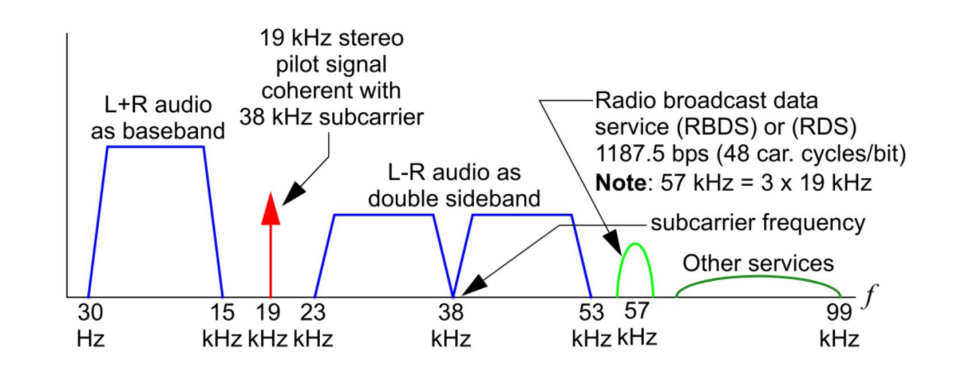
\includegraphics[width=0.8\textwidth]{fm_channel_freq_content.png}
\caption{Frequency spectrum of a typical FM broadcast signal, showing the baseband audio (0--15 kHz), stereo pilot tone (19 kHz), and stereo difference signal (23--53 kHz).}
\label{fig:fm_spectrum}
\end{figure}

\section*{Lab Overview}
In this laboratory session, we implemented a real-time FM demodulation system using an RTL-SDR dongle and MATLAB. The objective was to receive FM broadcast signals, demodulate them, and play the resulting audio through the computer's speakers in real time. We developed two implementations: one using MATLAB's built-in \texttt{comm.FMBroadcastDemodulator} System object (\texttt{main1.m}) and another with a custom FM demodulator based on phase differentiation and filtering (\texttt{main2.m}). The custom demodulator required us to design low-pass filters and adjust the frame length to optimize audio quality, revealing a trade-off between processing latency and signal fidelity.

\section*{Implementation Details}

\subsection*{Implementation 1: Using MATLAB's Built-in Demodulator (\texttt{main1.m})}
The first implementation utilized MATLAB's Communication System Toolbox to configure a real-time FM radio receiver. The system parameters were defined as follows: center frequency of 93.5 MHz, sampling rate of 240 kHz, and audio sampling rate of 48 kHz. The \texttt{comm.SDRRTLReceiver} System object was used to acquire complex I-Q samples from the RTL-SDR dongle, with a frame size of 10,240 samples. Automatic Gain Control (AGC) was disabled, and a fixed tuner gain of 50 was set to ensure consistent signal strength.

A \texttt{dsp.SpectrumAnalyzer} was configured to visualize the power spectrum of the received signal in real time, aiding in debugging and signal analysis. The \texttt{comm.FMBroadcastDemodulator} object performed FM demodulation with a frequency deviation of 75 kHz, converting the I-Q samples to an audio signal at 48 kHz. The demodulated audio was played using an \texttt{audioDeviceWriter} object. The main processing loop continuously acquired frames, normalized the I-Q samples, visualized the spectrum, demodulated the signal, and played the audio.

\begin{lstlisting}[caption={Main processing loop in \texttt{main1.m}},label={lst:main1}]
while true
    iq = double(radio());
    iq = iq / max(abs(iq)); % Normalize
    specAnalyzer(iq);
    audio = fmDemod(double(iq));
    player(audio);
end
\end{lstlisting}

\subsection*{Implementation 2: Custom FM Demodulator (\texttt{main2.m})}
The second implementation replaced the built-in demodulator with a custom FM demodulation function. Two low-pass FIR filters were designed using the \texttt{designfilt} function:
\begin{itemize}
    \item \textbf{First filter}: A low-pass filter with a passband frequency of 100 kHz and stopband frequency of 120 kHz to isolate the FM signal within the desired bandwidth.
    \item \textbf{Second filter}: A low-pass filter with a passband frequency of 15 kHz and stopband frequency of 17 kHz to extract the mono (L+R) audio signal after demodulation.
\end{itemize}
The demodulation process involved:
1. Normalizing the received I-Q samples.
2. Filtering the signal with the first low-pass filter to remove out-of-band noise.
3. Computing the instantaneous phase using \texttt{unwrap(angle(...))}.
4. Differentiating the phase to obtain the frequency-modulated signal.
5. Removing the DC component by subtracting the mean.
6. Filtering the demodulated signal with the second low-pass filter to isolate the audio.
7. Decimating the signal by a factor of 5 (from 240 kHz to 48 kHz) to match the audio playback rate.
8. Playing the resulting audio using \texttt{audioDeviceWriter}.

The frame size was increased to 14,336 samples (1024$\times$14) to improve audio quality by providing more samples for filtering, which better approximated the signal's spectral power density.

\begin{lstlisting}[caption={Main processing loop in \texttt{main2.m}},label={lst:main2}]
while true
    % -- getting the envelope signal --
    iq = double(radio());
    iq = iq / max(abs(iq)); % Normalize
    filteredSignal = filter(lpFilt, iq);
    % -- getting the phase, differentiating it & removing its DC --
    instPhase = unwrap(angle(filteredSignal));
    demodulated = diff(instPhase);
    demodulated = demodulated - mean(demodulated);
    filteredSignal2 = filter(lpFilt2, demodulated);
    % -- decimation of L+R signal --
    decimation_factor = fs / audioFs; % =5 here
    audio = decimate(filteredSignal2, decimation_factor);
    audio = audio / max(abs(audio));
    % -- playing the L+R signal --
    player(audio);
end
\end{lstlisting}

\section*{Trade-off Analysis}
In \texttt{main2.m}, increasing the frame size from 10,240 to 14,336 samples improved the audio quality by allowing the filters to process more data, resulting in a closer approximation of the signal's spectral power density. This was particularly noticeable in reduced noise and clearer audio output. However, this came at the cost of increased processing latency, as larger frames required more time to filter and process. The trade-off highlights the balance between computational load and signal fidelity in real-time systems. Compared to \texttt{main1.m}, the custom demodulator in \texttt{main2.m} produced slightly lower audio quality due to the simplicity of the phase differentiation approach and potential mismatches in filter design, but it provided valuable insight into the FM demodulation process.

\section*{Conclusion}
This lab demonstrated the implementation of a real-time FM demodulation system using RTL-SDR and MATLAB. The first approach (\texttt{main1.m}) leveraged MATLAB's built-in tools for robust and efficient demodulation, while the second approach (\texttt{main2.m}) required custom filter design and phase differentiation, revealing practical challenges in real-time signal processing. The trade-off between frame size, processing latency, and audio quality was a key learning outcome, emphasizing the importance of optimizing system parameters for real-time applications.

\end{document}
